\experiment{Deadlock detection}{11/10/2023}

\section{Aim}
Implement the algorithm for deadlock detection.

\section{Algorithm}
\begin{enumerate}
   \item Start
   \item Input the number of processes and resource types.
   \item Input available resources, allocation matrix, and request matrix.
   \item Initialize the work matrix.
   \item For each process 'i', check if all its allocation entries are zero. If yes, set the corresponding 'finish' entry to 1.
   \item Loop through all the processes and check if they can be executed:
   \begin{enumerate}
       \item Loop through all the processes again to find a process that has not finished yet.
       \item Check if the remaining resources needed by the process are less than or equal to the available resources.
       \item If the process can be executed, mark the process as finished.
   \end{enumerate}
   \item Print the safe sequence.
   \item Stop
\end{enumerate}

\section{C Program}
\begin{lstlisting}[label={list:c_program:queue}]
#include <stdio.h>

int available[10], work[10], allocation[10][10], req[10][10], finish[10], flag = 0;

void main() {
    int n, m;

    printf("Enter the number of processes: ");
    scanf("%d", &n);

    printf("Enter the number of resource types: ");
    scanf("%d", &m);

    printf("\nEnter available resources: ");
    for (int i = 0; i < m; i++) {
        scanf("%d", &available[i]);
    }

    printf("\nEnter allocation matrix:\n");
    for (int i = 0; i < n; i++) {
        printf("Process %d: ", i);
        for (int j = 0; j < m; j++) {
            scanf("%d", &allocation[i][j]);
        }
    }

    printf("\nEnter request matrix:\n");
    for (int i = 0; i < n; i++) {
        printf("Process %d: ", i);
        for (int j = 0; j < m; j++) {
            scanf("%d", &req[i][j]);
        }
    }

    for (int i = 0; i < m; i++) {
        work[i] = available[i];
    }

    for (int i = 0; i < n; i++) {
        flag = 0;
        for (int j = 0; j < m; j++) {
            if (allocation[i][j] != 0) {
                flag = 1;
                break;
            }
        }
        if (flag == 0)
            finish[i] = 1;
        else
            finish[i] = 0;
    }

    for (int i = 0; i < n; i++) {
        for (int j = 0; j < n; j++) {
            if (finish[j] == 0) {
                flag = 0;
                for (int k = 0; k < m; k++) {
                    if (req[j][k] > work[k]) {
                        flag = 1;
                        break;
                    }
                }
                if (flag == 0) {
                    for (int l = 0; l < m; l++)
                        work[l] += allocation[j][l];
                    finish[j] = 1;
                }
            }
        }
    }

    flag = 0;
    for (int i = 0; i < n; i++) {
        if (finish[i] == 0) {
            flag = 1;
            printf("\nDeadlock detected!\n");
            break;
        }
    }

    if (flag == 0)
        printf("\nNo deadlock\n");
}
\end{lstlisting}

\section{Output}
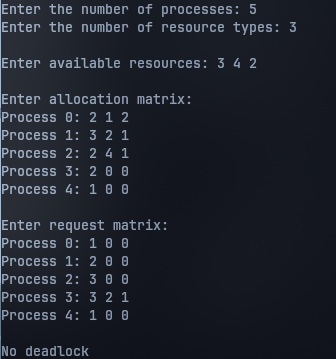
\includegraphics[]{Cycle_4//Outputs/deadlock.png}
\newpage
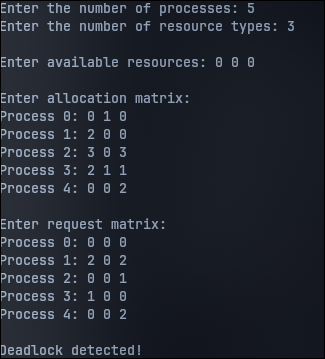
\includegraphics[]{Cycle_4//Outputs/deadklock1.png}



\section{Result}
Executed deadlock detection algorithm successfully